\chapter{Исследовательская часть}

\section{Технические характеристики}

Технические характеристики устройства, на котором выполнялось тестирование:

\begin{itemize}
	\item операционная система: Windows 10;
	\item оперативная память: 16 Гб;
	\item процессор: Intel® Core™ i5-8259U;
	\item количество ядер: 4;
	\item количество логических процессоров: 8.
\end{itemize}

Во время тестирования ноутбук был включен в сеть питания и нагружен только встроенными приложениями окружения и системой тестирования.


\section{Сравнение времени выполнения реализаций алгоритмов}

Сравнивалось время работы (обычное, по таймеру) последовательной стандартизации данных и стандартизации с использованием параллельного конвейера.  Эти реализации сравнивались по времени обработки заявок на стандартизацию массива вещественных чисел из 10000 элементов в зависимости от количества заявок: 1, 5, 25 и от 50 до 250 с шагом 50. 
 
Так как некоторые задачи выполняются достаточно быстро, а замеры времени имеют некоторую погрешность, они для каждой реализации и каждого количества заявок выполнялись 10 раз, а затем вычислялось среднее время работы.
 

На рисунке \ref{img:time_all} приведены результаты сравнения времени выполнения реализаций алгоритмов. 

\img{120mm}{time_all}{Сравнение времени работы реализаций в зависимости от количества заявок}


Как и ожидалось, параллельная реализация выполняется за меньшее количество времени в сравнении с линейной за счет того, что в ней одновременно на разных лентах (потоках) обрабатываются несколько заявок. Причем с ростом числа заявок разрыв между реализациями увеличивается.


\section{Анализ статистики параллельного конвейера}

На рисунке \ref{fig:stats} приведен результат сбора статистики при обработке 1000 заявок на обработку массива из 100000 элементов.

\newpage
\begin{figure}[h!]
	
	\centering{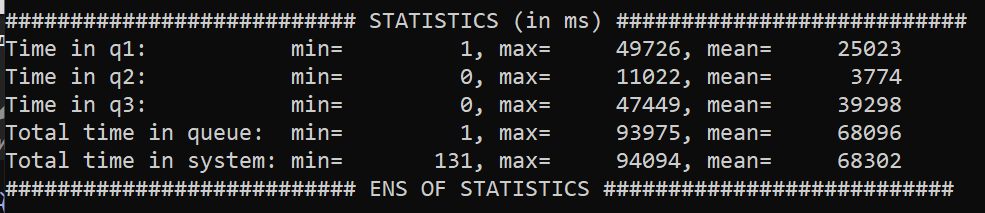
\includegraphics[scale=1]{inc/img/stats.png}}
	
	\caption{Результат сбора статистики}
	
	\label{fig:stats}
	
\end{figure}


Как видно из рисунка, очереди с наибольшим максимальным временем нахождения в них заявки -- первая и третья.
 Для первой очереди такой результат объясняетсяя тем, что она заполняется генератором заранее, и последняя заявка находится в ней до того момента, пока все предшествующие ей не будут обработаны первой лентой. Это подтверждает и среднее время, проведенное заявкой в первой очереди, которое приблизительно равно половине от максимального.
 
 Для третьей же очереди наибольшее максимальное (и, в частности, среднее) время нахождения в ней заявки связано со сложностью работы соответсвующей ей ленты. Она преобразовывает исходный массив, записывая полученные в результате вычитаний и делений новые значения в результирующий массив, на что тратится большое количество операций и, соовтетсвенно,  время.


Минимальное время нахождения заявки в каждой очереди соответсвует отметкам первой задачи: в каждую ленту она попадает сразу же, не ожидая окончания обработки в этом потоке предыдущей задачи. 

Вычитая из минимального времени, проведенного заявкой в системе, минимальное суммарное время, проведенное заявкой в очередях, можно вычислить время обработки этой заявки, равное 130 мс.

При этом можно заметить, что минимальное, максмальное и среднее время, проведенное заявкой в системе слабо  отличается от тех же замеров для времени, проведенного заявкой в очередях. Это, а также анализ времени, проведенного заявками в третьей очереди,  еще раз подтверждает, что при организации параллельного конвейера необходимо разбивать задачу на этапы, схожие по трудоемкости, иначе большую часть времени заявки будут простаивать в очередях.


\section{Вывод из исследовательской части}

Таким образом, параллельная организацияя обработки данных с использованием конвейера  работает быстрее, чем линейная обработка. При этом для достижения наилучших показателей необходимо корректно разделять задачу на этапы: так, чтобы время их выполнения было приблизительно равным, иначе большую часть времени заявки будут простаивать в очереди наиболее трудоемкой ленты.